Um sistema multiagente (SMA) organizado é aquele constituído por agentes autônomos que interagem visando um propósito em comum, tendo como consequência um comportamento global \cite{moiseframework,organiationofmultiagentsystem}. Assim sendo, uma organização com essas características deve ser capaz de manifestar conhecimento em comum, cultura, memória, história, distribuição de atividades e a capacidade de distinguir um  agente em específico \cite{organiationofmultiagentsystem}. Deste fato é possível identificar o fenômeno \textit{supra-individual} que implica em um comportamento que existe além dos comportamentos e atributos particulares no que diz respeito as entidades constituintes do sistemas. 

Uma organização de um sistema multiagente deve conter relações sociais no que tange a agentes, institutos e grupos sociais \cite{organiationofmultiagentsystem}. Também deve apresentar uma \textit{extensão de um espaço abstrato}. Isso implica uma representação dos seguintes conceitos: estrutura espacial, estrutura temporal, símbolos, semântica e capacidade de dedução. Há organizações que não se enquadram em todas essas restrições, contudo são suficientes para tratar o problema dentro de uma perspectiva computacional \cite{organiationofmultiagentsystem}.

A subseção \textit{Conceitos Gerais de uma Organização de Sistemas Multiagentes} tem por finalidade, detalhar melhor os elementos presentes da Teoria da Organização dentro do contexto de SMA em relação a esse estudo. Já a subseção \textit{Formalização de Conceitos Específicos para SMA} tem por objetivo realizar uma verificação analítica dos elementos presentes no modelo de \textit{SMA} denominado por \textit{MOISE+}. Os conceitos que serão analisados são: objetivos, planos e papéis \cite{organiationofmultiagentsystem}.
   

\subsection{Conceitos Gerais de uma Organização de Sistemas Multiagentes}

A finalidade desta subseção consiste em trabalhar com uma maior riqueza de detalhes, todos os conceitos que constituem a ideia de uma organização de um sistema multiagente. Esses conceitos estão estruturados no texto que se segue.
  
\textbf{Divisão em tipos de atividades:} uma organização não é uniformemente estruturada. Isso, pois as atividades são distribuídas de forma desigual entre as diferentes entidades. Dentro do ponto de vista fenomenológico as atividades estão sujeitas a classificação, e ocorrem com diferentes frequências e em diferentes regiões dentro das definições espaciais da organização \cite{organiationofmultiagentsystem}.

\textbf{Integração:} dentro de uma organização ocorre a presença de interdependência entre diferentes espaços de atividades. Essas, por sua vez, estão relacionadas em uma estrutura única definida dentro de um contexto alinhado e integrado \cite{organiationofmultiagentsystem}.

\textbf{Composição:} uma organização é composta por elementos menores. No caso de uma \textit{SMA}, os elementos atômicos que estruturam a organização são os agentes \cite{organiationofmultiagentsystem}.

\textbf{Estabilidade/Flexibilidade:} uma organização apresenta padrões de atividades. Esses padrões possuem características que podem ser enquadradas em dois aspectos: estáveis e flexíveis. No que tange as características estáveis, essas são constituídas por elementos/processos que definem o padrão em si mesmo. Em contraste com isso um comportamento flexível acontece quando o sistema é submetido a situações incomuns \cite{organiationofmultiagentsystem}.

\textbf{Coordenação:} todo sistema é dependente de algum recurso. Assim sendo, é preciso que esse recurso seja utilizado de forma inteligente a fim de que possa se manter ao longo do tempo. Para isso, se faz necessário que a organização se comporte como uma amplificadora de recursos a fim de que as estruturas operacionais tenham um comportamento cada vez mais organizado \cite{selforganization, selforganizatioenvoriment, defintionselforganization}. Contudo as incertezas relacionadas aos efeitos combinados resultam em influências negativas nas eficiências. Portanto, para manter a eficiência organizacional se faz necessário a existência de elementos otimizadores sobre os padrões de atividades \cite{organiationofmultiagentsystem}.

\textbf{Recursividade:} uma organização é constituída por sub-organizações. Isso ocorre em diferentes níveis de estrutura e se dá por intermédio de um padrão recursivo \cite{organiationofmultiagentsystem}.

\textbf{Representação Multi-Nível e Causalidade:} a natureza recursiva das organizações resultam em atividades ocorrendo em diferentes escalas espaciais, temporais e estruturais. Como consequência disto, as cadeias causais presentes em estruturas organizacionais são processos multi-níveis \cite{organiationofmultiagentsystem}.

\textbf{Potenciais e Diferenciais:} diversos são os sistemas físicos onde as forças entre partículas são decorrentes de balanços de potenciais. Como esse comportamento está presente em diversos sistemas físicos, existem modelos abstratos de sistemas auto-organizáveis que levam em consideração a presença de forças potenciais e diferenciais em organizações \cite{selforganizationdiffforce}. Esse conceito é trabalhado dentro de sistemas multiagentes. Um exemplo notório é o conceito de \textit{Poder}, o qual é entendio como a capacidade de influenciar uma organização \cite{organiationofmultiagentsystem}.

\textbf{Regras e Gramáticas:} organizações podem ser compreendidas como potenciais configurações de atividades e processos. Essas configurações podem ser descritas usando gramática \cite{grammarselforganizationmodel,grammarselforganizationmodel2}. Tanto as gramáticas como as regras que compõem uma organização apresentam três interpretações, que são: como estruturas (especificações procedurais do que deve ser feito): como coação (as ações são definidas no que pode e não pode ser feito) e como um compilado das experiências \cite{organiationofmultiagentsystem}.

\textbf{Incerteza:} não é possível conceber o conceito de uma organização sem ao menos entendê-la como uma estrutura que distribui informação em si mesma. Sob esta ótica, a distribuição de informação inequivocamente implica geração de incerteza o que por sua vez se manifesta como um complicante no que tange a comunicação entre as partes bem como a atividade organizacional em si mesma.

\subsection{Formalização de Conceitos Específicos para SMA}
\label{moiseformalizesma}
A apresentação desses conceitos será feita por intermédio de estudos relacionados ao \textit{MOISE+}. Apesar de ser um arcabouço, o \textit{MOISE+} trata a rigor acadêmico na ótica da computação clássica a tratativa dada para os conceitos em interesse a esse estudo. Assim sendo, uma análise aprofundada do modelo, bem como dos textos em referência, satisfazem com excelência os fundamentos teóricos para os estudos em desse texto. 

A constituição do \textit{MOISE+} é estruturada em três categorias de especificação, essas são: estrutural, funcional e deôntica. 

A especificação estrutural acontece em três níveis: individual: social e coletivo. O nível individual trata de definir os papéis $\rho$ dos agentes. A hereditariedade é uma relação que se dá entre dois papéis em que se $\rho'$ é filho de $\rho$ então $\rho'$ é uma especialização de $\rho$. Um exemplo apropriado para isso é o jogo de futebol onde existe o papel jogador dado por $\rho$ e existe o papel atacante dado por $\rho'$ \cite{moiseframework,roleone,roletwo,dynamicagenttemporalstruct}. Em termos formais, essa relação é dada por: 

\begin{eqnarray}
\rho_a \sqsubset \rho_b
\end{eqnarray}

O nível social estabelece relações de ligação dados pelo predicado $link(\rho_s,\rho_d,t)$. Existem três possíveis valores para $t$, os quais são $t = \{aut, com, acq\}$. O valor $auth$ significa autoridade (neste caso $\rho_s$ exerce autoridade sobre $\rho_d$), o valor $com$ significa comunicação (neste caso $\rho_s$ pode se comunicar com $\rho_d$) e o valor $acq$ significa conhecimento ($\rho_s$ tem conhecimento da existência de $\rho_d$) \cite{moiseframework,dynamicagenttemporalstruct}. O MOISE+ define as seguintes relações de implicabilidade

\begin{eqnarray}\nonumber
	link(\rho_s,\rho_d,auth) \to link(\rho_s,\rho_d,com) \nonumber \\
	link(\rho_s,\rho_d,com) \to link(\rho_s,\rho_d,acq) 
\end{eqnarray}

O modelo também determina como se dão as relações de hereditariedade para o predicado de $link$ \cite{moiseframework,dynamicagenttemporalstruct}: 

\begin{eqnarray}\nonumber
	link(\rho_s,\rho_d,t) \wedge \rho_s' \sqsubset \rho_s' \to link(\rho_s',\rho_d,t) \nonumber \\
	link(\rho_s,\rho_d,t) \wedge \rho_d' \sqsubset \rho_d' \to link(\rho_s,\rho_d',t) 	
\end{eqnarray}


O nível coletivo determina a existência de compatibilidade entre os papéis \cite{moiseframework}. Essa é uma relação reflexiva e o seu conceito se dá através da seguinte proposição: Se papel $\rho_a$ possui a capacidade de realizar um determinado objetivo, então o papel $\rho_b$ também tem essa capacidade. Em termos formais, essa relação se dá da seguinte forma \cite{moiseframework,deonticOne}:

\begin{eqnarray}
	\rho_a \bowtie \rho_b \wedge \rho_a \neq \rho_b \wedge \rho_a \sqsubset \rho' \to \rho' \bowtie \rho_b 
\end{eqnarray}

O nível coletivo também apresenta o conceito de grupo dado por $gt$ o qual é constituído por:

\begin{eqnarray}
	gt = \langle R,SG,L^{intra},L^{inter},C^{intra},C^{inter},np,ng\rangle 
\end{eqnarray}

Em que $R$ é o conjunto dos papéis não abstratos, $SG$ são subgrupos que estão contidos neste grupo, $L^{intra}$ consiste dos $links$ intra-grupos, $L^{inter}$ dos links inter-grupos, 
$C^{intra}$ das relações de compatibilidade intra-grupos e $C^{inter}$ das relações de compatibilidade inter-grupos. O símbolo $np$ denota a cardinalidade mínima e máxima para uma dada 
função e o símbolo $ng$ realiza o mesmo para os subgrupos \cite{moiseframework}. 

A Especificação Funcional tem a finalidade descrever os objetivos a serem atingidos dentro de uma estrutura de árvore. A Figura \ref{arvoremoise} a seguir define como se dá esse tipo de especificação: 

\begin{figure}[H]
  \centering
  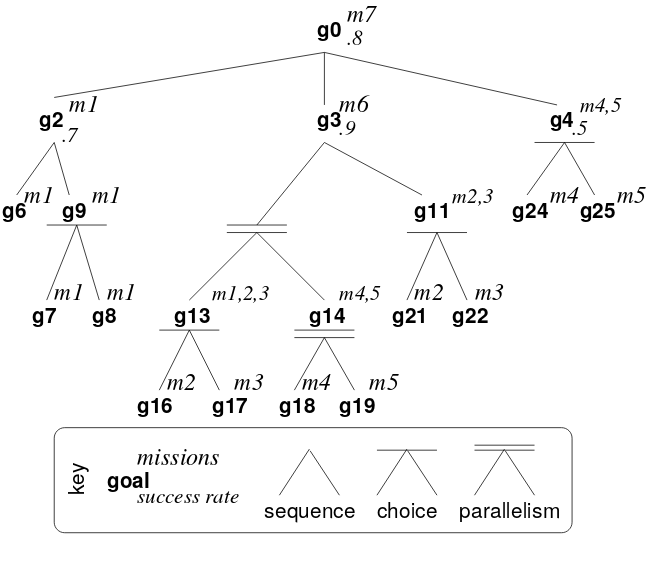
\includegraphics[width=0.8\linewidth]{figure/figmoise} 
  \caption{Árvore de objetivos definido pelo modelo MOISE+ \cite{moiseframework}}
  \label{arvoremoise}
\end{figure}

A Figura \ref{arvoremoise} define três tipos de relação de sub-objetivos: $sequence$ onde todos os sub-objetivos devem necessariamente ser concluídos em sequência: $choice$ onde o agente tem a possibilidade de escolher qual objetivo ele deseja seguir, e $parallelism$ onde todos os objetivos devem ser concluídos, contudo sem uma sequência definida \cite{taems01,taems02}. Esta parte do modelo é baseada em um arcabouço de distribuição de atividades denominado por \textit{TAEMS} \cite{TAEMS}. 

Como é possível observar na Figura, os objetivos são agrupados em conjuntos de missões $m$ \cite{dynamicagenttemporalstruct}. A relação a seguir define isso melhor:

\begin{eqnarray}
	m_k = \{ g_n,...,g_m\}
\end{eqnarray}


A Especificação Deôntica define predicados para estabelecer permissões e obrigações entre os papéis e as missões. Toda obrigação implica necessariamente em uma permissão, conforme define a relação a seguir \cite{moiseframework,deonticOne}: 

\begin{eqnarray}\nonumber \label{deonticRuleMoise}
	obl(\rho,m,tc) \to per(\rho,m,tc) \\
	obl(\rho,m,tc) \wedge \rho \sqsubset \rho' \to obl(\rho',m,tc) \\
	per(\rho,m,tc) \wedge \rho \sqsubset \rho' \to per(\rho',m,tc) \\	
\end{eqnarray}

Onde o predicado $obl$ define uma obrigação e o predicado $per$ define permissão. O argumento $tc$ define uma periodicidade de tempo para o qual a relação deôntica é valida. 